\documentclass[12pt,a4paper]{article}
\usepackage{cmap}
\usepackage[T2A]{fontenc}
\usepackage[utf8]{inputenc}
\usepackage[russian,english]{babel}
\usepackage{amsmath,amssymb}
\usepackage[pdftex]{color,graphicx}
\usepackage{float,indentfirst}
\usepackage[format=hang,labelsep=endash]{caption}
\usepackage[unicode,colorlinks,linkcolor=blue,
        bookmarks,bookmarksnumbered]{hyperref}
\usepackage{tikzsymbols}
\usepackage{tikz}
\usetikzlibrary{arrows,shapes,patterns}
\tikzset{>=latex'}

\usepackage{geometry}
  \geometry{left=3cm}
  \geometry{right=3cm}
  \geometry{top=2cm}
  \geometry{bottom=2cm}
\usepackage{xurl}

\begin{document}

\title{CS index}
\author{E.V.Eremin \texttt{<e.v.eremin>}}

\maketitle

\begin{abstract}
Computer science topics index.
\end{abstract}

\section{Introduction}

What should be known.

\section{People}

List of people who asked right questions.

\begin{itemize}
\item Pythagoras of Samos (Пифагор) c.~570 – c.~495~BC
\item Socrates
\item Plato (Platon)
\item Aristotle (Aristoteles)
\item Euclid
	\begin{itemize}
	\item Elements
	\end{itemize}
\item Leonard Euler
\item Лев Николаевич Толстой
\item Claude E. Shannon
	\begin{itemize}
	\item A Symbolic Analysis of Relay and Switching Circuits, 1937.
	\end{itemize}
\item Edsger Wybe Dijkstra (E. W. Dijkstra)
\item Donald Knuth
	\begin{itemize}
	\item The Art of Computer Programming, 1962, ...
	\item \TeX
	\item MIX, MMIX
	\end{itemize}
\item Robert Sedgewick
\item Dennis Richie,
\item Brian Kernigan
\item Alfred Aho
\end{itemize}

\section{Hardware}

\begin{itemize}
\item Computer Organization and Design by David Patterson
\item Operating Systems: Three Easy Pieces

    Remzi H. Arpaci-Dusseau and Andrea C. Arpaci-Dusseau

    \url{https://pages.cs.wisc.edu/~remzi/OSTEP/}

\item Operating System Principles

    CSE 30341 is the one of the core classes in the Computer Science and 
    Engineering program at the University of Notre Dame.

    \url{https://www3.nd.edu/~pbui/teaching/cse.30341.fa17/}

\item Linkers and Loaders by John R. Levine,

    Published by Morgan-Kauffman in October 1999, ISBN 1-55860-496-0

    \url{https://www.iecc.com/linker/}
    \url{https://linker.iecc.com/}

\end{itemize}

\textbf{References}

\subsection{Central Processing Unit (CPU)}

\begin{itemize}
\item Pipeline
\item Branch Prediction
\item Memory Hierarchy
\end{itemize}

\subsubsection{Co-processors, Arithmetic Accelerators, Math Units}

\begin{itemize}
\item MMX, SSE, AVX, Neon, etc.: SIMD-instructions
\end{itemize}

\subsubsection{Instruction Execution}

\section{Virtual Memory and Memory Management}

\subsection{Memory Segments}

\subsection{MMU and Paging}

\begin{itemize}
\item PGD (Page Global Directory)
\item PUD (Page Upper Directory)
\item PMD (Page Middle (Mid-level) Directory)
\item PTE (Page Table Entry)
\item Page
\end{itemize}

\begin{itemize}
\item PAE (Physical Address Extension)
\item Page Frame.  Physical memory is organized into \emph{page frames}.  The 
size of a page frame is a power of 2 in bytes and varies among systems.
\item Page.  Logical memory is organized into \emph{pages}. The size of page 
matches a page frame.
\item PFN (Page Frame Number).  A PFN is simply an index within physical memory 
that is counted in page-sized units. PFN for a physical address could be 
trivially defined as (\verb"page_phys_addr >> PAGE_SHIFT").
\end{itemize}

\begin{enumerate}
\item Four-level page tables merged [Posted January 5, 2005 by corbet]

    \url{https://lwn.net/Articles/117749/}

\item Mel Gorman (mel at skynet dot ie).  Understanding the Linux Virtual Memory Manager

    \url{https://www.kernel.org/doc/gorman/}
\end{enumerate}

\subsubsection{Stack}

\begin{itemize}
\item Stack pointer
\item Frame pointer
\item Jump/Branch and Return Instructions
\end{itemize}

\subsubsection{Interrupts and Interrupt Handling}

\subsection{CPU Cache}

\begin{figure}[H]
\begin{center}
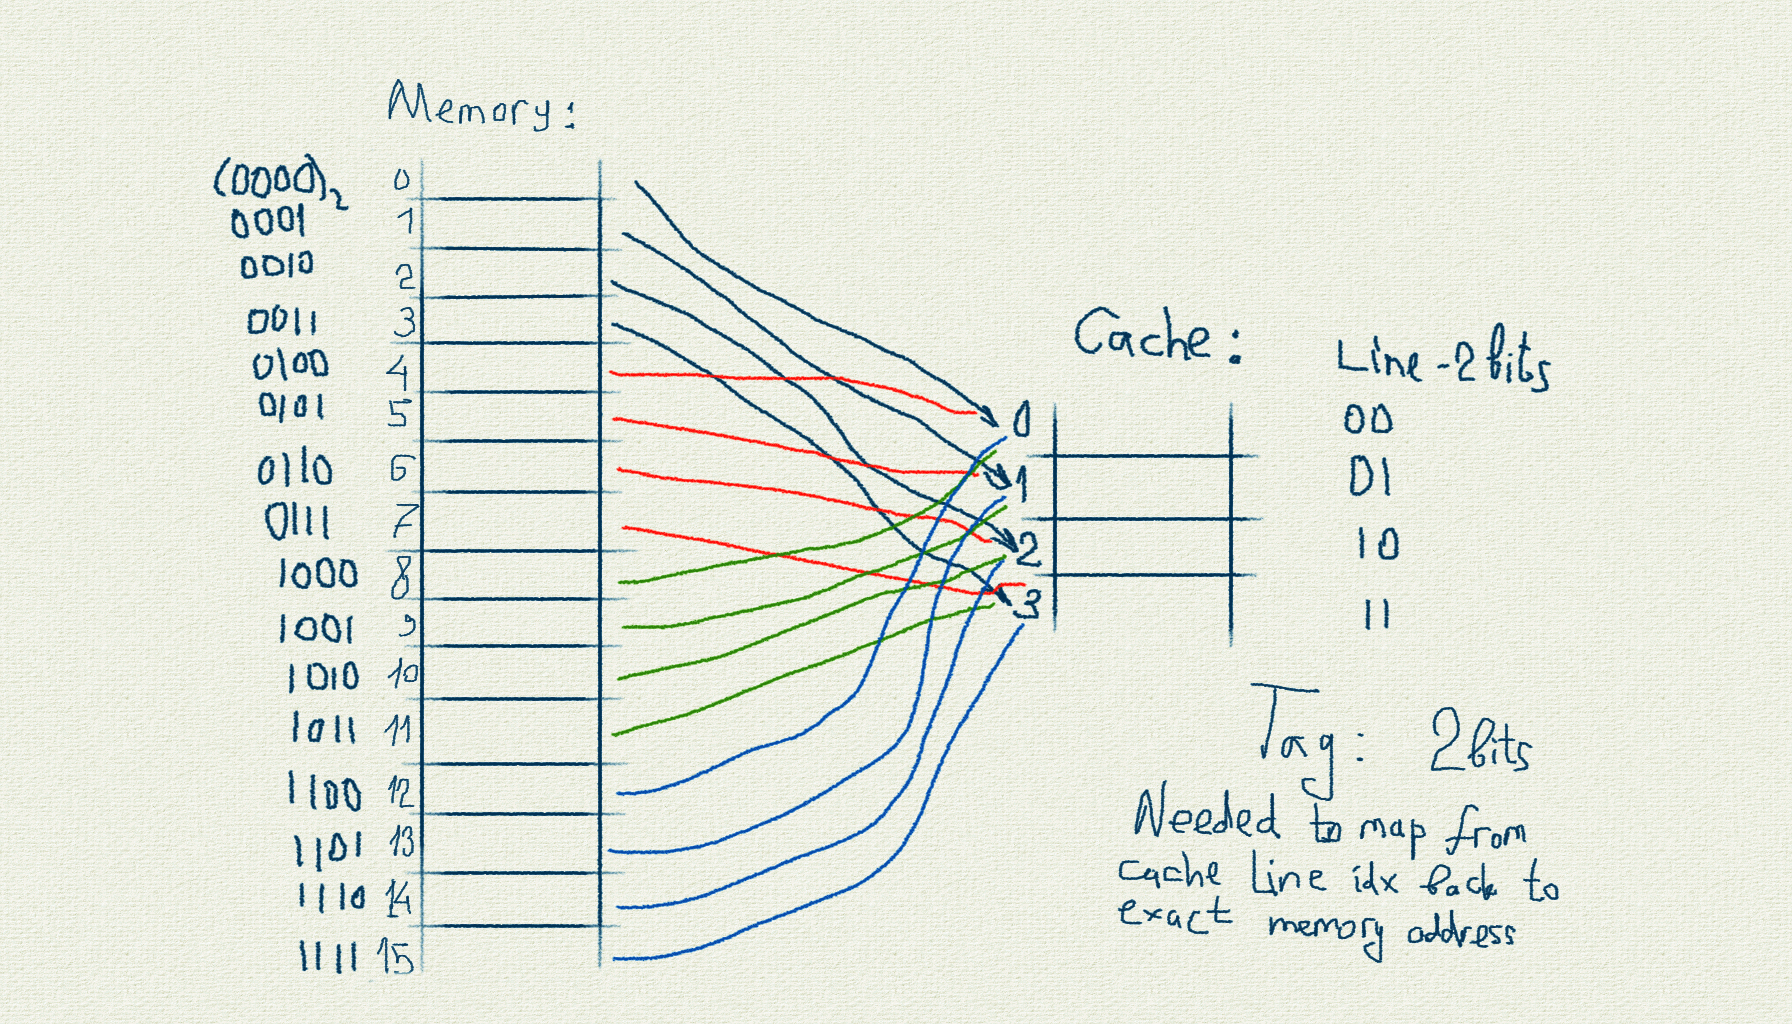
\includegraphics[width=1\textwidth]{png/cache-direct.png}
\caption{CPU Cache Direct Mapping}\label{fig.cache-direct-mapping}
\end{center}
\end{figure}

\begin{itemize}
\item Direct Mapping
\item Associative Mapping
\item Set-Associative Mapping

    \begin{itemize}
    \item One-way associative
    \item N-way associative
    \end{itemize}

\item Cache Coherence
\end{itemize}

\textbf{References}

\subsection{Page-replacement algorithm}

\begin{enumerate}
\item Least Recently Used (LRU)
\end{enumerate}

\subsection{References}

\begin{enumerate}
\item CSE 240A: Graduate Computer Architecture

	\begin{enumerate}
    \item Cache (CSE240A-MBT-L15-Cache.ppt.pdf)

        \url{https://cseweb.ucsd.edu/classes/fa10/cse240a/pdf/08/}

    \item Virtual Memory (CSE240A-MBT-L18-VirtualMemory.ppt.pdf)

        \url{https://cseweb.ucsd.edu/classes/fa10/cse240a/pdf/08/}

    \end{enumerate}

\item CSE378: Machine Organization \& Assembly Language

    \begin{itemize}
    \item How do caches work?

        \url{https://courses.cs.washington.edu/courses/cse378/09wi/lectures/lec15.pdf}

    \end{itemize}

\end{enumerate}

\subsection{Multiprocessing}

\subsection{TLS}

\section{Software}

\subsection{Shared Libraries/Object}

\begin{figure}[H]
\begin{center}
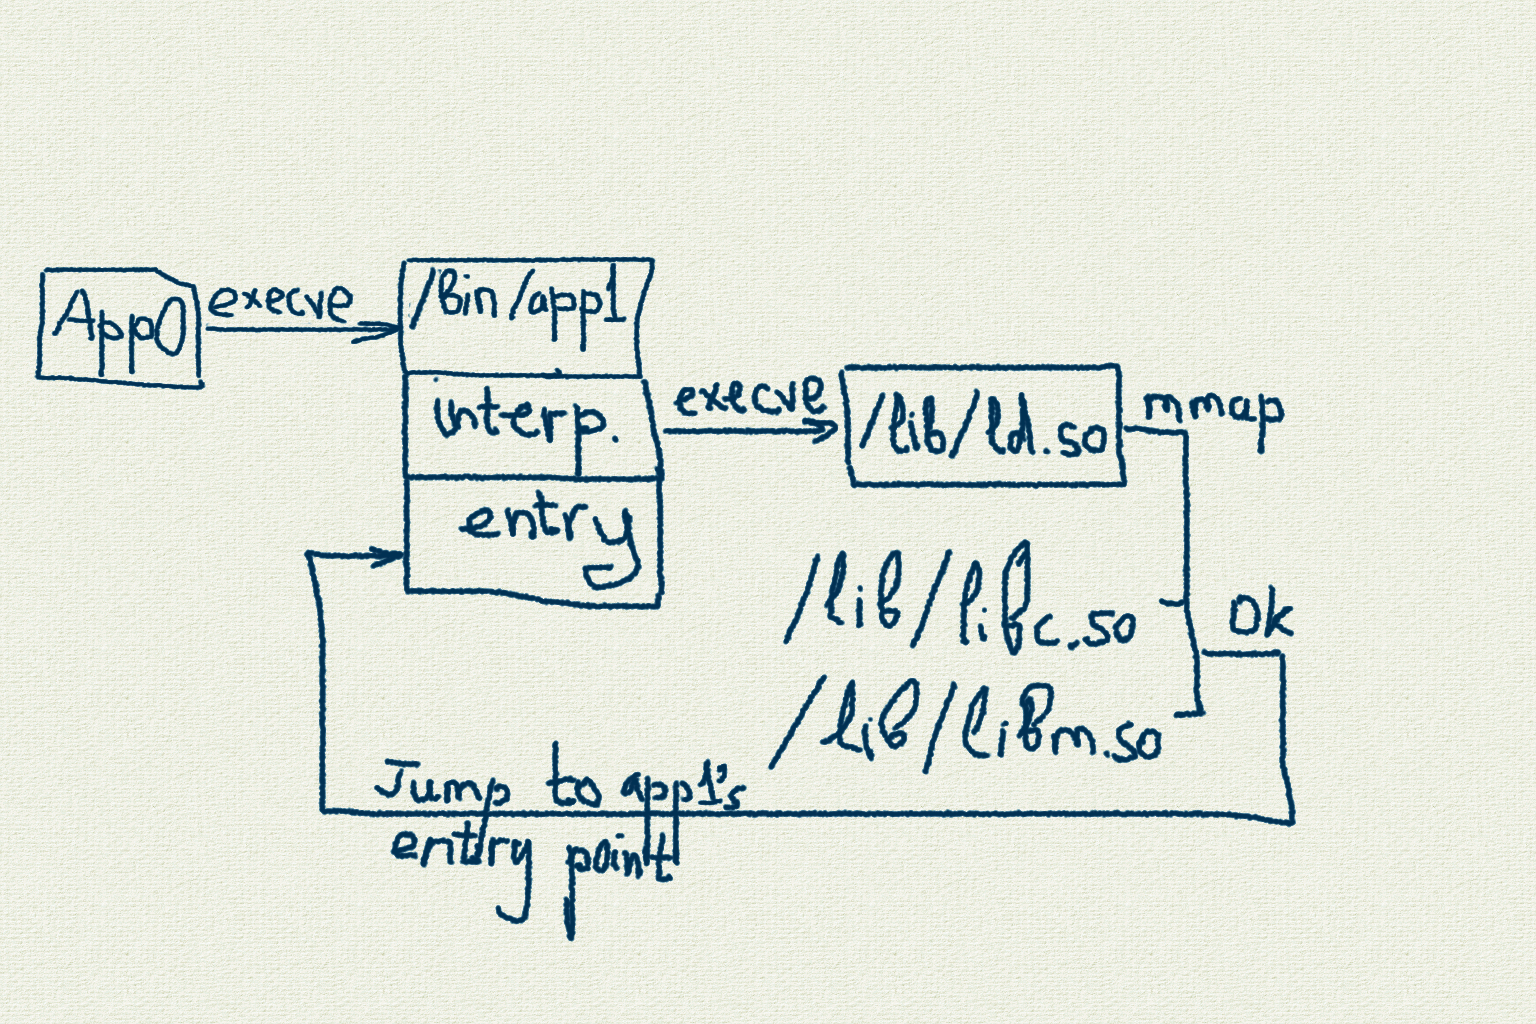
\includegraphics[width=1\textwidth]{png/ld.so.png}
\caption{How an executable using shared libraries is 
loaded}\label{fig.execve-ld.so}
\end{center}
\end{figure}

\textbf{References}

\begin{itemize}
\item Ulrich Drepper \url{<drepper@gmail.com>},
      How To Write Shared Libraries,
      December 10, 2011

      \url{https://www.akkadia.org/drepper/dsohowto.pdf}

\end{itemize}

\subsection{Subprograms/Routines/Functions}

\begin{itemize}
\item Subroutine/Subprogram
\item Subroutine Argument Passing
\item Return Address
\item Static
\item Thread-safe
\item Re-entrant
\end{itemize}

\subsection{Bit Manipulation/Twiddling}

\textbf{References}

\begin{enumerate}
\item Hacker's Delight by Henry S. Warren, Jr (2002, 2013)

\item Bit Twiddling Hacks by Sean Eron Anderson \url{<seander@cs.stanford.edu>}

    \small
    \url{https://graphics.stanford.edu/~seander/bithacks.html}

\end{enumerate}

\subsection{Locking}

\begin{itemize}
\item futex
\item mutex
\item spinlock
\item rwlock (Reader/Writer Lock)
\item RCU
\item Semaphores
\end{itemize}

\subsubsection{RCU (Read, Copy, Update)}

RCU --- Read, Copy, Update.

Paul McKenney series on LWN.net:

\begin{enumerate}
\item What is RCU, Fundamentally?

    \url{https://lwn.net/Articles/262464/}

\item What is RCU? Part 2: Usage

    \url{https://lwn.net/Articles/263130/}

\item RCU part 3: the RCU API

    \url{https://lwn.net/Articles/264090/}

\item The RCU API, 2019 edition

    \url{https://lwn.net/Articles/777036/}

\end{enumerate}

\section{Tracing and Profiling}

\begin{enumerate}
\item Dynamic Tracing
\item ftrace
\begin{verbatim}
mount -t tracefs tracefs /sys/kernel/tracing
\end{verbatim}
\item KProbes
\item Perf
\end{enumerate}

\section{Debugging and Instrumenting}

\subsection{GDB}

\subsection{Valgrind}

\section{Virtualization}

\subsection{QEMU}

\subsection{VirtualBox}

\subsection{Namespaces}

\begin{enumerate}
\item Separation Anxiety: A Tutorial for Isolating Your
      System with Linux Namespaces

    \url{https://www.toptal.com/linux/separation-anxiety-isolating-your-system-with-linux-namespaces}

\end{enumerate}

\subsection{lxc}

\subsection{lxd}

\subsection{Docker}

\section{memcpy}

\begin{itemize}
\item memcpy

	\begin{itemize}
	\item Overlapped memory regions/blocks
	\end{itemize}

\item memmove
\end{itemize}

\textbf{References}

\section{Software Engineering}

\subsection{Compatibility}

\begin{enumerate}
\item Backward compatibility
\item Forward compatibility
\end{enumerate}

\subsection{Frameworks}

\subsubsection{GLib}

\subsubsection{GTK+}

\subsubsection{Boost}

\subsubsection{Qt}

\textbf{References}

\begin{enumerate}
\item QThreads general usage

	\url{https://wiki.qt.io/QThreads_general_usage}

\item Maya Posch, How To Really, Truly Use QThreads; The Full
      Explanation, November 1, 2011

    Threads in an operating system are a very simple thing. Write a function, 
    maybe bundle it with some data and push it onto a newly created thread.  
    Use a mutex or other method to safely communicate with the thread if 
    necessary.  Whether it are Win32, POSIX or other threads, they all 
    basically work the same and are quite fool-proof. I’d venture to say that 
    they’re at least a lot easier to use and handle than sockets \Smiley 
    $\stackrel{..}{\smallsmile}$

	\small
    \url{https://mayaposch.wordpress.com/2011/11/01/how-to-really-truly-use-qthreads-the-full-explanation/}

\item Integrating QML and C++

	\url{https://doc.qt.io/qt-5/qtqml-cppintegration-topic.html}

\item Interacting with QML Objects from C++

	\url{https://doc.qt.io/qt-5/qtqml-cppintegration-interactqmlfromcpp.html}

\item D-Pointer

	\url{https://wiki.qt.io/D-Pointer}

\end{enumerate}

\section{Command Line Interface (CLI)}

\subsection{Vim}

Configuration files:

\begin{itemize}
\item \verb"$HOME/.vimrc"
\end{itemize}

\subsubsection{\$HOME/.vimrc}

\begin{verbatim}
set keymap=russian-jcukenwin
set iminsert=0
set imsearch=0
set spelllang=ru_yo,en_us

set hlsearch
set si
set ic
set fo=tcqro

highlight lCursor guifg=NONE guibg=Cyan
highlight clear SpellBad
highlight SpellBad cterm=underline

map <unique> <F2> a<C-R>=strftime("%Y.%m.%d-%H:%M:%S")<CR><CR><Esc>
map <unique> <F10> :emenu Encoding.<TAB>
map <unique> <F5> :w<CR>:make<CR>

set wildmenu
set wcm=<Tab>
menu Encoding.KOI8-R :e ++enc=8bit-koi8-r<CR>
menu Encoding.cp1251 :e ++enc=8bit-cp1251<CR>
menu Encoding.ibm-866 :e ++enc=8bit-ibm866<CR>
menu Encoding.UTF-8 :e ++enc=2byte-utf-8 <CR>

" Only do this part when compiled with support for autocommands.
if has("autocmd")
  " When editing a file, always jump to the last known cursor position.
  " Don't do it when the position is invalid or when inside an event handler
  " (happens when dropping a file on gvim).
  autocmd BufReadPost *
    \ if line("'\"") >= 1 && line("'\"") <= line("$") |
    \   exe "normal! g`\"" |
    \ endif
endif " has("autocmd")

" vim highlight a matching parenthesis/brace
hi MatchParen cterm=none ctermbg=green ctermfg=blue

" syntax highlight and filetypes
let myfiletypefile = "~/.vim/filetype.vim"
filetype on
syntax on
\end{verbatim}

\subsection{Bash}

Configuration files:

\begin{verbatim}
${HOME}/.bashrc
${HOME}/.bash_profile
${HOME}/.profile
/etc/bashrc
/etc/profile
\end{verbatim}

\subsection{\$HOME/.bashrc}

Ignore duplicated commands and those which begin with a space (\verb"ignoreboth"
= \verb"gnorespace", \verb"ignoredups"), save more history.

\begin{verbatim}
HISTCONTROL=ignoreboth
HISTSIZE=100000
HISTFILESIZE=2000000
\end{verbatim}

Set Vim as the default editor.

\begin{verbatim}
export EDITOR=vim
\end{verbatim}

Set man page text width to 80 characters.

\begin{verbatim}
export MANWIDTH=80
\end{verbatim}

Git shortcuts.

\begin{verbatim}
alias gil='git log --stat'
alias gig='git grep'
alias gis='git status'
alias gid='git diff'
alias gib='git branch'
alias gia='git add'
alias gic='git commit -v'
alias gif='git log --graph --format="%C(auto)%h %ad %cd %d %ae %s"'
\end{verbatim}

Make \texttt{rm} (remove), \texttt{mv} (move) and \texttt{cp} (copy) commands less dangerous.

\begin{verbatim}
alias rm='rm -i'
alias mv='mv -i'
alias cp='cp -i'
\end{verbatim}

\subsection{Readline}

Configuration file:

\begin{verbatim}
inputrc
\end{verbatim}

Set incremental history search:
\begin{verbatim}
"\e[A": history-search-backward
"\e[B": history-search-forward
\end{verbatim}

\verb"\e[A" means \verb"Up", \verb"\e[B" means \verb"Down".  To find out other 
bindings just run \verb"read" Bash command and press any key, e.g. Home:
\begin{verbatim}
$ read
^[[1~
\end{verbatim}

Here \verb"^[" prefix means \verb"Escape", so the sequence for \verb"Home" must 
be replaced with \verb'"\e[1~"' in inputrc file.

\textbf{References}

\begin{enumerate}
\item unix.stackexchange.com: What is the general format of keyname for key 
bindings in “inputrc” file?

	https://unix.stackexchange.com/questions/24132/what-is-the-general-format-of-keyname-for-key-bindings-in-inputrc-file
\end{enumerate}

\subsection{Vim}

\begin{verbatim}
.vimrc
\end{verbatim}

Fix random syntax highlighting breaks

\begin{verbatim}
:syntax sync fromstart
:syntax sync minlines=20
\end{verbatim}

\subsection{Git}

Configuration files:

\begin{verbatim}
.git/config

$(HOME)/.git/config
\end{verbatim}

Change tags color in 'git log' and similar (yellow on white is a bit hardly 
readable):
\begin{verbatim}
# color.decorate.tag
[color "decorate"]
    tag = magenta

[user]
    name = E.V.Eremin
    email = e.vl.eremin@yandex.ru
    username = eremin
\end{verbatim}

\subsubsection{Github (or similar)}

Generating an SSH key

\begin{verbatim}
$ ssh-keygen -t rsa -b 4096 -C 'e.vl.eremin@yandex.ru'
$ xclip -sel clip < ~/.ssh/id_rsa.pub
$ git remote add origin 'git@github.com:eremin-ev/cs-idx.git'
\end{verbatim}

\subsection{Tmux}

Configuration file:

\begin{verbatim}
tmux.conf
\end{verbatim}

Example:

\begin{verbatim}
set-option -g prefix C-a
unbind-key C-b
bind-key C-a send-prefix

# Shift arrow to switch windows
bind -n F11  previous-window
bind -n F12 next-window

# status bar
set-option -g status-interval 60
set-option -g status-left-length 30
set-option -g status-style bg=green,bold,fg=white
#set -g window-status-style bg=black
set-option -g window-status-current-style bg=white,fg=black
set-option -g window-status-current-format "[#I:#W#F]"
#set -g window-status-current-fg black
#set -g window-status-current-attr bold
#set -g status-left '#[fg=green,bg=white](#S)'
set-option -g status-right '#[default] #[fg=white]%H:%M#[default]'
\end{verbatim}

\subsection{Screen}

\begin{verbatim}
screenrc
\end{verbatim}

\section{Conclusion}

Write your conclusion here.

\begin{equation}
    \label{simple_equation}
    \alpha = \sqrt{\beta}
\end{equation}

\end{document}

% vim:spell:fo+=aw:
